\documentclass[adraft, copyright, creativecommons]{eptcs} % TODO: Change to submission at the end
\providecommand{\event}{TERMGRAPH 2022} % Name of the event you are submitting to
% \usepackage{breakurl}             % Not needed if you use pdflatex only.
\usepackage{underscore}           % Only needed if you use pdflatex.

% My packages
\usepackage{orcidlink} % Orcid links
\newcommand\Mark[1]{\textsuperscript#1}

% Footnotes inside tables
\usepackage{footnote}
\usepackage{glossaries} % Glossary
\makesavenoteenv{tabular}
\makesavenoteenv{table}
\usepackage[nameinlink]{cleveref} % Reference footnotes.
\crefname{figure}{{figure}}{figures}
\Crefname{figure}{{Figure}}{Figures}
\crefformat{footnote}{#2\footnotemark[#1]#3}
% Math
\newtheorem{definition}{Definition}
\newcommand{\definitionautorefname}{Definition}
% Acronyms
\newacronym{bpmn}{BPMN}{Business Process Modeling Notation}

\title{BPMN semantics formalization and \\ model checking using graph grammars}
\author{Tim Kräuter\Mark{*}\orcidlink{0000-0003-1795-0611}, \quad
Harald König\Mark{\textdagger}\Mark{*}\orcidlink{0000-0001-6304-6311}, \quad
Adrian Rutle\Mark{*}\orcidlink{0000-0002-4158-1644}, \quad
Yngve Lamo\Mark{*}\orcidlink{0000-0001-9196-1779}
\institute{
\Mark{*}Western Norway University of Applied Sciences, Bergen, Norway
}
\institute{
\Mark{\textdagger}University of Applied Sciences, FHDW, Hannover, Germany}
\email{tkra@hvl.no, harald.koenig@fhdw.de, aru@hvl.no, yla@hvl.no}
}
\def\titlerunning{BPMN semantics formalization and model checking using graph grammars}
\def\authorrunning{Kräuter \textit{et al.}}
\begin{document}
\maketitle

% Maximum 8 pages for the first extended abstract!
% At the end, 15 pages for the proceedings.

% TODO: Semantics vs. execution semantics?

\begin{abstract}
TBD abstract
\end{abstract}

\section{Introduction}
\begin{itemize}
    \item State goals: Semantics formalization/reference implementation
    \item Easy BPMN model checking (definition of propositions using BPMN syntax!)
\end{itemize}

\section{Semantics formalization}
% \begin{itemize}
%     \item General approach: Model transformation from any BPMN file to a graph grammar. Rules are generated specifically for each file.
%     \item Go through the BPMN spec and explain the formalization similar to the structure in \cite{vangorpVisualTokenbasedFormalization2013}.
%     \item Talk about best practices that help explain why some elements have not been formalized yet (Problems with the inclusive gateway, complex gateway, etc.).
% \end{itemize}
% General approach
We have developed a novel approach to cover as many of the \gls*{bpmn} features as possible.
Our approach is summarized as a \gls*{bpmn} process model in \cref{fig:approach}.
It is based on a model transformation from \gls*{bpmn} process models to graph grammars.
Thus, our approach is \textit{generative}, i.e., it constructs a new graph grammar including rules and a start graph for each \gls*{bpmn} process model.
This is a major difference compared to other approaches such as \cite{corradiniFormalApproachAnalysis2021, vangorpVisualTokenbasedFormalization2013} where only the \gls*{bpmn} process model is transformed but the rewrite rules are fixed.
\begin{figure}[h]
    \centering
    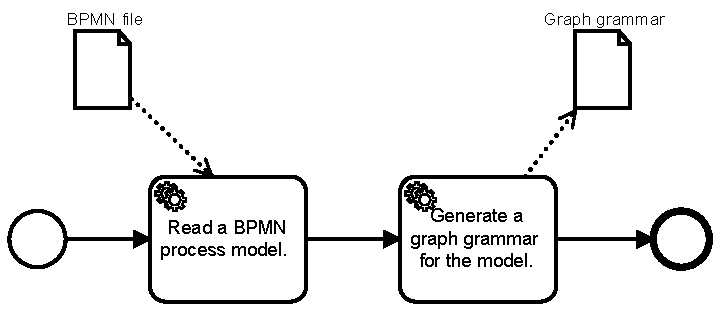
\includegraphics[width=0.5\textwidth]{images/approach-first-part.pdf}
    \caption{Semantics generation by model transformation}
    \label{fig:approach}
\end{figure}

We will now shortly introduce graph grammars before we explain the \gls*{bpmn} execution semantics formalization in detail following a similar structure as the \gls*{bpmn} specification \cite[Chapter 13]{objectmanagementgroupBusinessProcessModel2013}.

\subsection{Graph grammars}
% Shortly introduce graph grammars.
% TODO: Self plagiarism!

% Graph grammar definition
\begin{definition}[Graph grammar] \label{def:graphGrammar}
A graph grammar $GG=(S, P)$ consists of a start graph $S$ and a set of production rules $P$ \cite{ehrigFundamentalsAlgebraicGraph2006}. 
\end{definition}

The idea of a graph grammar is to begin with a start graph and then continuously apply all possible production rules.
Thus, one obtains a state space where each state is a graph, and each transition is a rule application.
Rules can be applied using different approaches, such as double-pushout (DPO) \cite{ehrigFundamentalsAlgebraicGraph2006} or single-pushout (SPO) \cite{loweAlgebraicApproachSinglepushout1993}.
Production rules for DPO are defined in \autoref{def:productionRule}.
Informally speaking, elements in $R$ but not in $L$ are added by a rule, while elements in $L$ and $R$ are preserved, and a rule deletes elements that are in $L$ but not in $R$.

% Rule definition
\begin{definition}[Production rule] \label{def:productionRule}
A production rule $P= L \overset{l}{\leftarrow} K \overset{r}{\to} R$ consists of graphs L, K, R, and graph morphisms $l: K \to L$ and $r: K \to R$ \cite{ehrigFundamentalsAlgebraicGraph2006}.
\end{definition}

% Rule application definition


% What about nested rules and NACS?

% Formalization
\subsection{Formalization}

\Cref{fig:bpmnfeaturesOverview} depicts the \gls*{bpmn} features supported by our approach.
It shows which events, gateways, activities and edges are included in the formalization.

% Describe which events are supported/ not supported. Not finalized yet
% Describe boundary events. Not finalized yet.

\begin{figure}[h]
    \centering
    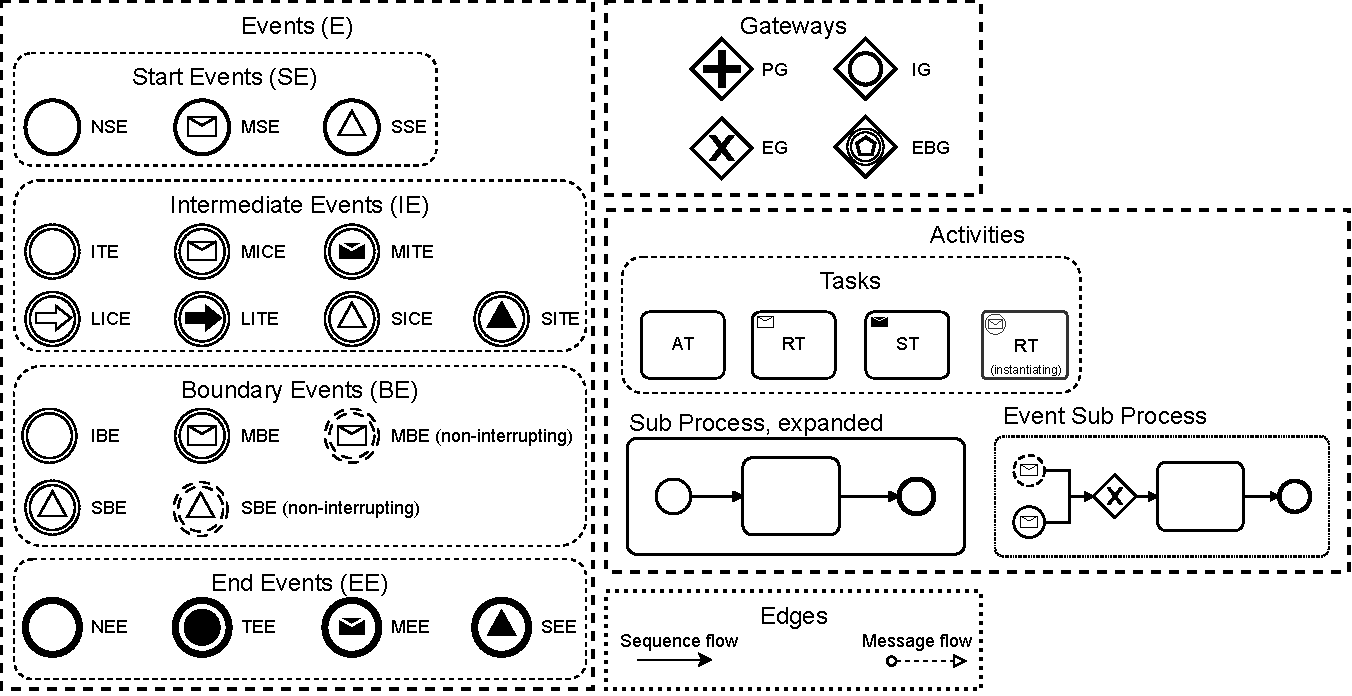
\includegraphics[width=0.8\textwidth]{images/bpmn_semantics-feature_overview.pdf}
    \caption{Overview of the supported \gls*{bpmn} features (structure adapted from \cite{houhouFirstOrderLogicVerification2022})}
    \label{fig:bpmnfeaturesOverview}
\end{figure}

% Describe which tasks are supported and that other tasks are meant by AT.
We support receive and send tasks which can be connected to each other or message events using message flows across different pools in a \gls*{bpmn} process model.
Receive tasks can instantiate a process instance if they do not have any incoming sequence flows and the \textsf{instantiating} property is set.
Other tasks such as service, user, script, business rule, manual and undefined tasks are handled uniformly.

% Describe supported sub processes.
Furthermore, we support two types of sub processes.
First, the occurrence of expanded sub processes in the sequence flow.
Second, the occurrence of event sub processes in pools.
Event sub processes can be started by message or signal start events either interrupting or non-interrupting.

% Describe gateways.
All gateways are supported besides the complex gateway.
However, the complex gateway is not used often \cite{freundRealLifeBPMNUsing2019} and not also not supported by other recent approaches \cite{corradiniFormalApproachAnalysis2021, houhouFirstOrderLogicVerification2022, vangorpVisualTokenbasedFormalization2013}.
% Describe edges. --> Default and conditional flows?

\subsubsection{Type graph}

\begin{figure}[h]
    \centering
    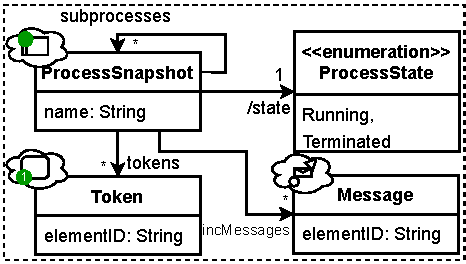
\includegraphics[width=0.5\textwidth]{images/bpmn_semantics-typegraph.pdf}
    \caption{BPMN execution type graph} % TODO: Cite my ecmfa paper?
    \label{fig:typeGraph}
\end{figure}

\subsubsection{Process instantiation and termination}

\subsubsection{Activities}
\subsubsection{Gateways}
% Exclusive gateway, parallel gateway, inclusive gateway, exclusive event based gateway
\subsubsection{Events}

% In the spec, this is below events
\subsubsection{Event Sub-Processes}

\section{Related work}
% Van gorp
A \gls*{bpmn} formalization based on in-place graph transformation rules is given in \cite{vangorpVisualTokenbasedFormalization2013}.
The formalization covers a substantial part of the \gls*{bpmn} specification, including complex concepts such as inclusive gateway merge and compensation.
In addition, graph transformation rules are visual and thus can easily be matched to the informal description of the execution semantics in the specification \cite{objectmanagementgroupBusinessProcessModel2013}.
The fixed set of graph transformation rules was implemented in a prototype using GrGen.NET.
Unfortunately, the implementation is not publicly accessible anymore.

% BProve/Corradini
The tool BProVe\footnote{\url{http://pros.unicam.it/bprove/}} is based on formal \gls*{bpmn} semantics given in rewriting logic and implemented in the Maude system.
Using these semantics, BProVe enables the verification of custom temporal properties for process models.
Furthermore, the tool is easily accessible online and includes multiple predefined properties, such as checking for dead activities and process completion \cite{corradiniBProVeToolSupport2017, corradiniFormalApproachAnalysis2021}.

% Houhou
The verification framework \textsf{fbpmn} uses first-order logic to formalize and check \gls*{bpmn} process models \cite{houhouFirstOrderLogicSemantics2019, houhouFirstOrderLogicVerification2022}.
This formalization is then realized in the TLA\textsuperscript{+} formal language and can be model-checked using TLC.
Their framework and related information is open source and freely available online\footnote{\url{https://github.com/pascalpoizat/fbpmn}}.
Similar to BProVe, \textsf{fbpmn} multiple beneficial predefined properties to be checked for process models.
However, they do not allow a user to define custom temporal properties.

Besides, these three approaches there are many more \gls*{bpmn} formalizations, for example, based on Petri Nets \cite{dijkmanSemanticsAnalysisBusiness2008} or process algebras \cite{wongProcessSemanticsBPMN2008}.
We picked them since they support a significant subset of the \gls*{bpmn} features, have easily accessible and well-documented tool support, and are pretty recent.

Nevertheless, different approaches support a different subset of the \gls*{bpmn} features, which impacts their usefulness in practical scenarios.
\Cref{tab:supportedFeatures} depicts which features of the \gls*{bpmn} execution semantics are supported by the different approaches and our approach.
% TODO: Check that this matches the BPMN spec and mention it

\begin{table}[htbp]
    \caption{Features supported by BPMN semantics (characterization based on \cite{vangorpVisualTokenbasedFormalization2013}).}
    \label{tab:supportedFeatures}
    \begin{tabular}{l l l l l}
    \hline
      Feature & Van Gorp &  Corradini & Houhou & This\\
      & et al. \cite{vangorpVisualTokenbasedFormalization2013} & et al. \cite{corradiniFormalApproachAnalysis2021}& et al. \cite{houhouFirstOrderLogicVerification2022} & paper\\
      \hline
      \textit{Instantiation and termination} & &\\
      Start event instantiation & X & X & X & X\\
      Exclusive event-based gateway instantiation & X & & & X\\
      Parallel event-based gateway instantiation &  & & & \\
      Receive task instantiation & & & & X\\
      Normal process completion & X & X & X & X\\
      \textit{Activities} & & & &\\
      Activity & X & X & X & X\\
      Subprocess & X & X* & X & X\\
      Ad-hoc subprocesses & & & &\\
      Loop activity & X & & & ?\\
      Multiple instance activity & & & & \\
      \textit{Gateways} & & & &\\
      Parallel gateway & X & X & X & X\\
      Exclusive gateway & X & X & X & X\\
      Inclusive gateway (split) & X & X & X & X\\
      Inclusive gateway (merge) & X & & X & X*\\
      Event-based gateway &  & X\footnote{Does not support receive tasks after event-based gateways.} & X & X\\ % No timer and conditional events after event based gateway supported.
      Complex gateway & & & &\\
      \textit{Events} & & & & \\
      None Events & X & & & X\\
      Message events & X & X & X & X\\
      Timer Events & & & X & X*\\
      Escalation Events & & & & \\
      Error Events (catch) & X & & & \color{yellow}X\\ % Yellow means I want to support this but not implemented yet.
      Error Events (throw) & X & & & \color{yellow}X\\
      Cancel Events & X & & & \color{yellow}X\\
      Compensation Events & X & & & \color{yellow}X\\
      Conditional Events & & & &\\
      Link Events & X & & & X\\
      Signal Events & X & & & X\\
      Multiple Events &  & & & \\
      Terminate Events & X & X & X & X\\
     Boundary Events & X\footnote{Only interrupting and } & & X\footnote{Message and timer events} & X\\ % To the same extent as the event support
      \textit{Event subprocess} &  &  &  & \\
      Message Start Event &  & & & X\\
      Message Start Event (non-interrupting) & & & & X\\
      Signal Start Event &  & & & X\\
      Signal Start Event (non-interrupting) &  & & & X\\
      Other Start Events &  & & & \\ % Conditional and Escalation.
    \end{tabular}
\end{table}

% Summarize the findings and explain them in more detail
% Explain Van Gorp in detail
Van Gorp et al. \cite{vangorpVisualTokenbasedFormalization2013} cover a large part of the \gls*{bpmn} semantics.
However, they do not support Event-based gateways and event subprocesses, while their support for boundary events is minimal.
Especially, Event-based gateways are often used and supported by every other approach.

% Explain Corradini in detail
Corradini et al. \cite{corradiniFormalApproachAnalysis2021} does only support message and terminate events.
However, many other types of events exist and are used in practice.
In addition, they do not support the occurrence of receive tasks after Event-based gateways.
Nevertheless, the same behavior can be achieved using message events.
% Limited subprocess support?

% Explain Houhou in detail
Houhou et al. only support message, timer, and terminate events.
However, they support the use of message and timer events as both interrupting and non-interrupting boundary events.
Their event support remains limited compared to other approaches.

% Explain our approach in more detail. What are we lacking?

% Our semantics should be the most complete to date
% Our semantics is also quite understandable.


% Our semantics is the only one that generates "rules" and not only converts the model to some representation, right?. So we are higher-order?
Besides semantics, our approach is also unique since it not only transforms a \gls*{bpmn} process model into a different representation but also generates graph-transformation rules for this specific model.
Other approaches, for example, rely on a fixed generic set of rules \cite{vangorpVisualTokenbasedFormalization2013} or Maude implementation \cite{corradiniFormalApproachAnalysis2021}.
% What about Houhou?
\section{Model checking BPMN}
Model-checking a \gls*{bpmn} process model is straightforward after a graph grammar describing its execution semantics has been generated.
\Cref{fig:modelChecking} depicts the inputs and outputs of model checking.

\begin{figure}[h]
    \centering
    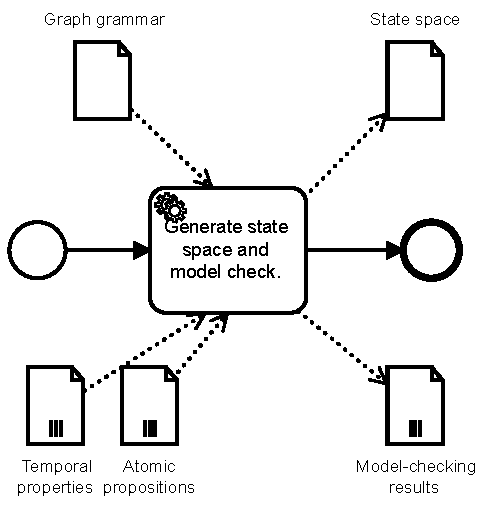
\includegraphics[width=0.4\textwidth]{images/approach-second-part.pdf}
    \caption{Model checking using graph grammars}
    \label{fig:modelChecking}
\end{figure}

Besides a graph grammar, a set of temporal properties to be checked and the atomic propositions used in the properties are supplied.
Atomic propositions must be formalized as graphs that can be matched to each state in the state space.
An atomic proposition holds in a state if and only if the graph associated with the atomic proposition is a subgraph of the graph associated with the state. % Cite groove/Rensink here.
This enables model checking of temporal properties using the defined atomic propositions.

% Defining atomic propositions in BPMN is a novelty.
Since we want to hide as much complexity as possible from a user who is model checking his \gls*{bpmn} process model, we let them define atomic propositions using the familiar \gls*{bpmn} syntax.
\gls*{bpmn} is usually explained and formalized using tokens, which flow through the process model.
Thus, to define an atomic proposition, we let the user attach tokens to his \gls*{bpmn} process model, which we can automatically convert to a graph condition.

For example, the token distribution shown in \cref{fig:atomicProposition} defines two running process instances with a token in task A/B.
Differently colored tokens belong to different process instances.
This visualization was significantly inspired by the excellent bpmn-js-token-simulation\footnote{\url{https://github.com/bpmn-io/bpmn-js-token-simulation}}.
% TODO: Implement this

% TODO: Change the picture to svg once implemented etc.
\begin{figure}[h]
    \centering
    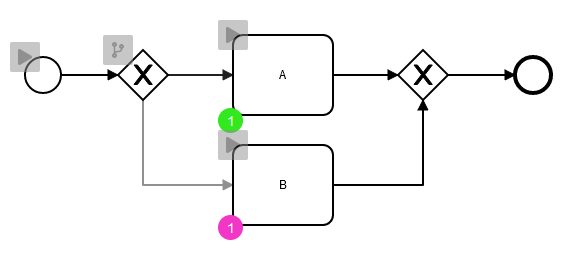
\includegraphics[width=0.6\textwidth]{images/atomicProposition.png}
    \caption{Token distribution defining an atomic proposition}
    \label{fig:atomicProposition}
\end{figure}

% TODO: We might look at some soundness things as in s3 and Bprove. Can we check them easily, and how?

\section{Implementation}
% \begin{itemize}
%     \item Talk about the tool implementation.
%     \item No installation should be needed.
%     \item Model transformation from BPMN to GG, concretely
%     \item Web tool which takes a BPMN-file and generates a zip containing a graph grammar for Groove to be downloaded, i.e.
%     \item The generated GG can be used for simulation and model checking in Groove.
%     \item We could also integrate an easier way to define atomic propositions directly using BPMN syntax and not in Groove.
% \end{itemize}
\subsection{Model-transformation to Groove}

\begin{figure}[h]
    \centering
    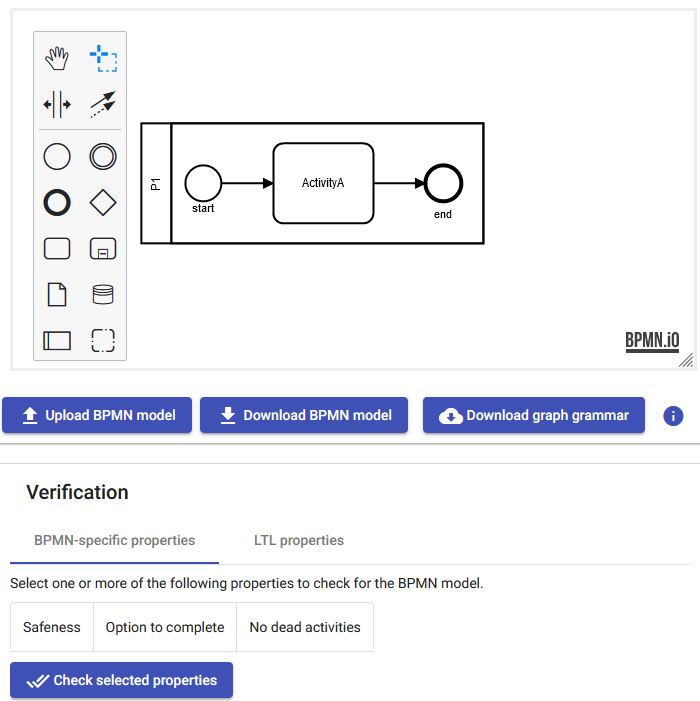
\includegraphics[width=1\textwidth]{images/impl.png}
    \caption{Implementation}
    \label{fig:impl}
\end{figure}

\subsection{Evaluation}
Evaluation using multiple test cases.

Add a table here which test cases cover what part of the semantics.
\section{Conclusion}

\bibliographystyle{eptcs}
\bibliography{bib} % TODO: Should be bib.
\end{document}
